% using Elseveir template per https://www.elsevier.com/authors/author-schemas/latex-instructions
\documentclass[review]{elsarticle}

\usepackage{lineno,hyperref}
\modulolinenumbers[5]

\journal{Journal of \LaTeX\ Templates}
\bibliographystyle{elsarticle-num}
\usepackage{booktabs}
\usepackage{graphicx}
\graphicspath{{../alt-ed-survey/figures-and-tables}}
\usepackage{hyperref}
\usepackage{threeparttable}  
\usepackage{tikz}
\usetikzlibrary{calc,matrix}

\begin{document}

\begin{frontmatter}

\title{
    % Comparative Policy Effects for Educational Diversity in Higher Education
    The Effect of H-1B and Section 127 Policy Interaction on Higher Education
    \tnoteref{titlenotes}
}
\tnotetext[titlenotes]{
    % Go to \url{https://github.com/Vandivier/research-dissertation-case-for-alt-ed/tree/master/papers/alt-ed-survey}
    % for additional materials including the online appendix,
    % survey data, and data analysis source code.
}

\author[mymainaddress]{John Vandivier} % \fnref{authorlinefootnote}}
\address[mymainaddress]{4400 University Dr, Fairfax, VA 22030}
\ead{jvandivi@masonlive.gmu.edu}

\begin{abstract}
    This paper estimates the policy effect on US higher education enrollment due to Section 127 employer educational assistance.
    This effect is estimated in two ways.
    First, by exploiting kinks in the amount employers may deduct for the purposes of educational assistance in 1978 and 1986.
    Secondly, real variation over time in the fixed nominal amount employers may deduct is assessed.
    Enrollment effects are decomposed by student salary to discover policies preferentially benefiting lower class and minority learners.
    Costs for encouraging lower class enrollment are compared between employer assitance and student loan approaches.
    Evidence suggests that [POLICY X] preferentially benefits lower and middle class individuals.
    % policy interaction with H-1B visa?
    % degree requirement as a strategy to import cheap, effective foreign labor (VISA)
    % this prevents high school graduates from directly entering roles that typically award section 127 (white color, major employer, corporate work)
    % until recently, that is, with walmart, mcdonalds, starbucks giving section 127 i think even to part timers
    % 1952 allows unlimited merit immigration, 1990 there is a quota and degree requirement added to H-1B: https://en.wikipedia.org/wiki/H-1B_visa#Immigration_Act_of_1990
    % New and initial H-1B and H-1B1 visas issued by the U.S. Department of State through consular offices
    % https://en.wikipedia.org/wiki/H-1B_visa#H-1B_visas_issued_per_year
    % crackdown in 2017: https://www.investopedia.com/news/impact-trumps-h1b-visa-crackdown-5-charts/
    % Theory: After 1990, companies began requiring a 4 year degree so they could have an H-1B justification.
    % This caused more americans to pursue an undergraduate degree without section 127. we should see section 127 use decline after 1990.
    % Recently, employers have begun giving the benefit anyway due to labor selection and internal ROI benefits
\end{abstract}

\begin{keyword}
education economics, alternative education, debt crisis, signaling
\MSC[2010] % TODO
\end{keyword}

\end{frontmatter}

\pagebreak
\linenumbers
        
        \section{Introduction and Description of Data}

        % maybe talk about stress and debt for why debt is important

        % NPSAS:19
        % Average undergraduate tuition and fees
        % for full-time students in all degree-granting postsecondary institutions,
        % by level and control of institution: Selected years, 1970-2016 [school year beginning 2016]
        % https://nces.ed.gov/programs/digest/d17/tables/dt17_330.10.asp
        % Constant 2016 dollars

        % inflation adjustment by PCE over time
        % https://fred.stlouisfed.org/series/PCE

        % 2016 is base year for corrected real deduction limit

        % Percentage of 18- to 24-year-olds enrolled in college,
        % by level of institution and sex and race/ethnicity of student: 1970 through 2017
        % https://nces.ed.gov/programs/digest/d18/tables/dt18_302.60.asp

        % college more diverse than ever https://www.aacu.org/aacu-news/newsletter/2019/march/facts-figures
        % more poor folks entering college https://www.insidehighered.com/news/2019/05/23/pew-study-finds-more-poor-students-attending-college
        % but can we do even better...? and not saddle them with debt? are these folks more in debt (higher debt load by status)...?

        % college board notes loans over time: https://research.collegeboard.org/trends/student-aid/figures-tables/total-federal-and-nonfederal-loans-type-over-time

        Welp, it seems not to have an important aggregate effect.
        We do know very few employees even use the benefit, ~5 percent.
        The local effect in 1970s seems very small or even negative, counter to prima facia economics
        If there's an effect at all it is for a small set of the population so it doesn't show in aggregate.
        Seems like loans are a much bigger effect.
        Actually this could still be interesting as it's prima facie an economic paradox
        % total enrollment: https://nces.ed.gov/programs/digest/d18/tables/dt18_303.10.asp
        % need employers offering the benefit over time.

        % what about student loans? here are the limits over time: https://www.finaid.org/loans/historicallimits.phtml
        % actual undergrad loans awarded since 1990 in the excel at https://research.collegeboard.org/trends/student-aid
        % but i don't think we should use actuals there bc that would explain away demand effects...we want to preserve those (do a better job explaining this plz)
        % so, prefer the limits over time...those are attributed to the school year, so rules beginning July 1993 are true for 1993 (start of school year)
        % eg dummy for "limit is subsidized plus unsubsidized" begins to be true for 1993 in my csv
        %
        % GI Bill accounting https://en.wikipedia.org/wiki/G.I._Bill#Chapter_30_(Montgomery_GI_Bill)
        % Variable implemented as categorical
        % [state A] original bill was 1944-1984
        % [state B] VEAP established 1981 https://www.benefits.va.gov/gibill/veap.asp
        % [state C] Montgommery GI went into effect 1984
        % [state D] Post-9/11 Montgomery GI Bill went into effect for 2009 school year https://www.thebalancecareers.com/gi-bill-for-the-21st-century-3347143
        % [state E] Forever GI bill rolls out new benefits starting in 2018 https://rebootcamp.militarytimes.com/education-transition/education/2017/08/16/trump-signed-the-forever-gi-bill-here-are-11-things-you-should-know/

        \section{Results}
        
        % \begin{table}
        %     \caption{Medium and Strong Models, Selected Variables}
        %     \begin{tabular}{lllll}
        %     Factor & 2018 Medium & 2018 Strong & 2019 Medium & 2019 Strong \\
        %     \toprule
        %     Male &  &  & -2.458* & -0.422** \\
        %     Not STEM & -1.269* \\
        %     X$_0$ & 1105.125 & .106 & -12345.347* & 3.289*** \\
        %     \bottomrule
        %     R-Squared & .597 & .504 & .526 & .319 %
        
        %     \end{tabular}
        %     \begin{tablenotes}
        %         \item{
        %             * p $<$ .05
        %             ** p $<$ .01
        %             *** p $<$ .001
        %         }
        %     \end{tablenotes}
        %     \label{tab:models}
        %     \end{table}
        
        % \begin{figure}[h!]
        %     \centering
        %     \caption{Employer Driven Favorability}
        
        %     \begin{tikzpicture}[element/.style={minimum width=1cm, minimum height=0.75cm}]
        
        %     \node (n1) [above=0.25cm] {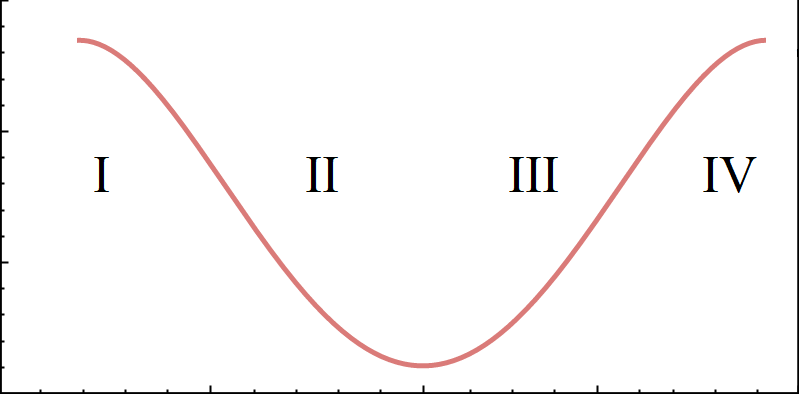
\includegraphics[width=0.5\textwidth]{../alt-ed-survey/figures-and-tables/figure-4.png}};
        %     \node (n2) [above=0.25cm] at ($(n1)!0.5!(n1) - (4, 1)$) {\rotatebox{90}{\textbf{Suitability}}};
        %     \node (n3) [above=0.25cm] at ($(n1)!0.5!(n1) - (0, 3)$) {\textbf{Time}};
        
        %     \end{tikzpicture}

        %     \label{fig:employer_driven_favorability}
        %     \end{figure}

        \section{Conclusions}
        
        % Pub. L. 99–514, § 1162(a)(2), substituted “$5,250” for “$5,000” in heading and twice in text
        % https://www.law.cornell.edu/rio/citation/Pub._L._99-514
        % https://www.ucop.edu/research-policy-analysis-coordination/_files/Public%20Law%2099-514.pdf
        % it moved 5000->5250 in 1986
        % can we see effect on median-and-below vs above?
        % important to look at wages not income (which would include investments, etc, see shrm's discussion: http://www.cpepea.com/wp-content/uploads/2017/05/10-0418-Coalition-Report-on-Public-Policy-Issue-E-P-E-A_FNL.pdf)
        % SHRM assessed only a single year, 2008. Shows Section 127 is mostly a Master's degree tool rn.
        % 75 percentile for salaries in 2017 was 54250 https://bizfluent.com/info-10032733-percentile-salary.html
        % define middle class as 50-75 percentile, lower class as under 50 percentile. break down effect by salary classification and see if it helps lower/middle
        % if so, it should improve diversity of education leading to a more diverse workforce which employers crave (TM) and politicians, etc...
        % Should we actually enact this policy? Effect on alternative credentials and credential inflation
        % Other options like extending the benefit to repayment https://blog.shrm.org/blog/let-s-fight-the-skills-gap-by-expanding-tax-free-education-assistance
        % we can also consider extending the education benefit to unaccredited education and income share agreements not just loans
        
        % https://www.nber.org/papers/w9225.pdf 
        % https://www.nber.org/digest/feb03/w9225.html

        \bibliography{./BibFile}
        
        \end{document}
        